\fancyhead[LE,RO]{Ionselective electrodes -- ,,SZEL''}
\fancyhead[LO,RE]{\thesection}
\fancyfoot[LE,RO]{\thepage}
\fancyfoot[RE,LO]{\emph{Physical chemistry laboratory practice}}

%\setcounter{section}{7}
\section{Determination of selectivity coefficient of ion-selective electrode}
\subsection{Introduction}

Ion-selective electrodes are potentiometric sensors, that allow the selective determination of the activity of certain ions.
They are widely used in the clinical diagnostics for routine measurements: automatic blood analisators measure the Na$^+$ and K$^+$-ion activity in blood samples. One more example is the determination of F$^-$-ion in tap water, even if there are interfering ions such as Cl$^-$ or OH$^-$. Their function is based on a selective membrane, which can be ionophore based (Na$^+$ and K$^+$), or lattice vacancy based (F$^-$). An example for the latter is the F$^-$ ion-selective electrode, which is based on a europium doped lanthanum fluoride crystal.

The equation that describes the behaviour of these electrodes is the Nernst-equation:

\begin{equation}
\label{eq:nernst}
	E
	=
	E^0
	+\frac{RT}{z_i F}
	ln(a_i)
\end{equation}

where $z_i$ is the signed valence of the primary ion (the ion that the electrode is selective to), $a_i$ is its activity.
According to the equation, for cation elective electrodes the electrode potential ($E$) is increasing with increasing actvity, and for anion selective ones, it decreases.
Because of deviations from the theoretical behaviour, in practice, we use the following, experimental equation:

\begin{equation}
\label{eq:exp}
	E
	=
	E^0
	\pm S ln(a_i)
\end{equation}

where $S$ is the slope of the linear part of the electrode calibration curve, which can be measured.
In real, multi-component samples, the potential of the ion-selective electrodes is influenced by the so-called \emph{interfering ions}, but in fact, more or less by every ion in the sample to some (small) extent.
For this reason, using eqs. \ref{eq:nernst} and \ref{eq:exp} will introduce error during evaluation.
To take into account these deviations we use the concept of \emph{selectivity coefficient} ($k_{pot}$). With this we can rewrite the equations as such: 

\begin{equation}
\label{eq:nikolsky}
E=E^0 + \frac{RT}{z_iF} \ln \left [ a_i + \sum_{j} \left ( k_{ij}a_j^{z_i/z_j} \right ) \right ]
\end{equation}

This is the Nikolsky equation. $a_j$ is the activity of the $j$th interfering ion, $z_j$ is its charge, $k_{pot}$ $i, j$ is the selectivity coefficient of the $j$th ion.
The selectivity coefficient shows how much more sensitive is the electrode towards the primary ion, then towards to the interfering ion.
For instance, if $k = 10^{-2}$, the activity of the $j$ ion must be hundredfold of the $i$ primary ion to have the same effect on the electrode potential (increase or decrease it to the same extent).
There are two main methods for determining the selectivity coefficient: the mixed and the separate solution methods.

In the mixed solution method, ion activity of the $j$ interfering ion is constant, and we increase the activity $i$ primary ion, and measure the potential response.
After plotting the data fig. \ref{fig:Q}, we find $Q$. Then, we calculate the selectivity coefficient as follows:

\begin{equation}
\label{eq:szel1}
	k_{i,j}^{pot}
	=
	\frac{(a_i^{z_j})_Q}{a_j^{z_i}}
\end{equation}


\begin{figure}
\centering
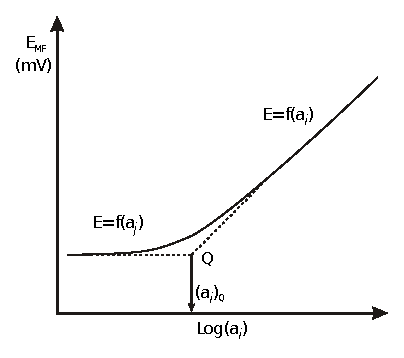
\includegraphics{fig/ion1.eps}
\caption{Using the mixed solution method to determine the selectivity coefficient.}
\label{fig:Q}
\end{figure}

When using the separate solution method, we need to record two calibration curves.
First, at zero interfering ion activity, we make a calibration of primary ion $i$, then at zero primary ion $i$ activity, we make a calibration plot of interfering ion $j$.
After obtaining these two curves, the selectivity coefficient can be obtained as seen in fig. \ref{fig:ion2}, taking either

\begin{enumerate}[(a)]
\item activities corresponding to the same potentials:

\begin{equation}
\label{eq:azonospot}
        k_{i,j}^{pot}
        =
        \frac{a_i}{a_j^{z_i/z_j}}
\end{equation}

\item or potentials corresponding to the same activities:

\begin{equation}
\label{eq:azonosakt}
        \lg k_{i,j}^{pot}
        =
        \frac{(E_2-E_1)zF}{2.303RT}
	=
	\frac{\Delta E}{S}
\end{equation}

\end{enumerate}

There are a number of factors that influence the selectivity coefficient: ionic strength, method, etc...
As it can be seen, from relationships \ref{eq:azonospot} and \ref{eq:azonosakt}, the drawback of the separate solution method is that it assumes, that the valence of the primary and interfering ion is equal, and that the sensitivity towards them is the same.
For this reason, selectivity coefficients obtained with this method are regarded as approximations, and the much better mixed solution method is preferred.

\begin{figure}
\centering
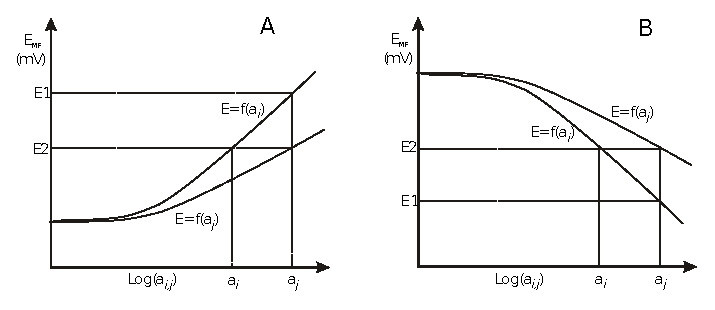
\includegraphics{fig/ion2.eps}
\caption{Determining the selectivity coefficient with the separate solution method for positive (A) and negative (B) ions.}
\label{fig:ion2}
\end{figure}

\subsection{Practice procedures}
The purpose of this practice is to study the function of potassium or fluoride ion-selective electrodes (ask the instructor which one).
Your first task is to prepare a dilution series of soluions of the primary ion. Use salts KCl or NaF.
Prepare 100 ml 10$^{-2}$ mol$\cdot$dm$^{-3}$ solution using a salt of the primary ion. 
Then make a tenfold dilution by taking out 10 ml from this solution, and putting it in another, clean 100 ml measuring flask. Fill it up to 100 ml with deionized water. Continue making dilution by always using the previous solutions, until you reach a concentration of 10$^{-6}$ mol$\cdot$dm$^{-3}$. 
Pour a small amount of each into separate, labeled beakers, so that the electrodes can submerse into them with their active area.
Then start with the most dilute solution by putting the measuring and the reference electrodes into it. Wait 1 minute, and write down the potential.
Move on to the next solution (10$\times$ more conc.), wait another 1 minute, and record the data.
Carry out measurements in all five solutions advancing from dilute to concentrated, repeat it altogether 3 times. Carefully rinse the electrodes between series.

\subsubsection{Determining the selectivity coefficient using the separate solution method}
Repeat the previous procedure, but use a salt of the interfering ion to prepare the first solution, the do the dilutions. It's important to use deionized water free of potassium, sodium, chloride and fluoride ions as much as possible. Ask the technician for ultrapure water. 

\subsubsection{Determining the selectivity coefficient using the mixed solution method}
For this method prepare another dilution series by using a salt of the primary ion, but instead of deionized water, use a 10$^{-2}$ M solution of the interfering ion as solvent. In this way, the interfering ion concentration will be constant in all of the solutions, but the primary ion concentration will vary just like in the first experiment.

\subsection{Evaluation}
\begin{enumerate}
\item Find the activity coefficients for the primary and interfering ions online, and calculate the activities from the concentrations.

\item Plot the $\lg a_i$ -- $E$ functions as seen in the diagrams above. 

\item Determine the slope of the linear part by linear fitting for each graph.

\item Determine the lower limit of detection of the electrode towards the primary ion ($Q$ when there is no interfering ion).

\item Calculate the selectivity coefficients using all 3 methods (1 mixed solution method and 2 separate solution methods).

\item For the separate solution method, plot the two curves in the same diagram.
\end{enumerate}

\subsection{Results to submit}
Lower limit of detecction towards the primary ion, 2 selectivity coefficients from the separate solution method, and 1 from the mixed solution method.
Five calibration diagrams, each with linear fits on the linear section.

\vfill
%\center
%Updated and translated by András Kiss assistant lecturer 2016.
